\documentclass{article}
\usepackage[utf8]{inputenc}
\usepackage{graphicx}
\usepackage{tabularx}
\usepackage[absolute]{textpos} % Para poner una imagen en posiciones arbitrarias
\usepackage{multirow}
\usepackage{float}
\usepackage{hyperref}
%\decimalpoint


\title{Métodos Computacionales}
\author{Tarea 2}
\date{Mayo de 2019}

\begin{document}

\maketitle
\section{Ejercicio 1: Fourier} 
\vspace{5mm}
\subsection{    Gráficas usando funciones signal y signalSuma.} 
\vspace{5mm}
\begin{center}
\includegraphics[width=10cm]{GarzonCamilo_signal_signalSuma.pdf} 

Figura 1. Grafica signal y signalSuma.
\begin{flushleft}
Se muestran las graficas de 2 señales, signal una funcion que esta dividida la primera mitad del dominio en una función y la segunda mitad en otro y signal suma que es una señal formada por la suma de dos señales senoidales.
\end{flushleft}
\includegraphics[width=10cm]{GarzonCamilo_TransformadasFourier_signal_signalSuma.pdf} 

Figura 2. Grafica transformada discreta de fourier de signal y signalSuma.
\begin{flushleft}
La transformada de Fourier de estas señales muestra como la potencia se concentra en distintos picos. Los picos de la fft de signal suma presentan una pendiente mayor que los picos de signal, esto puede ser debido a los cambios de amplitud mas suaves en la funcion signal. Tambien se pude observar que la distancia entre los picos en ambos casos es la misma.
\end{flushleft}
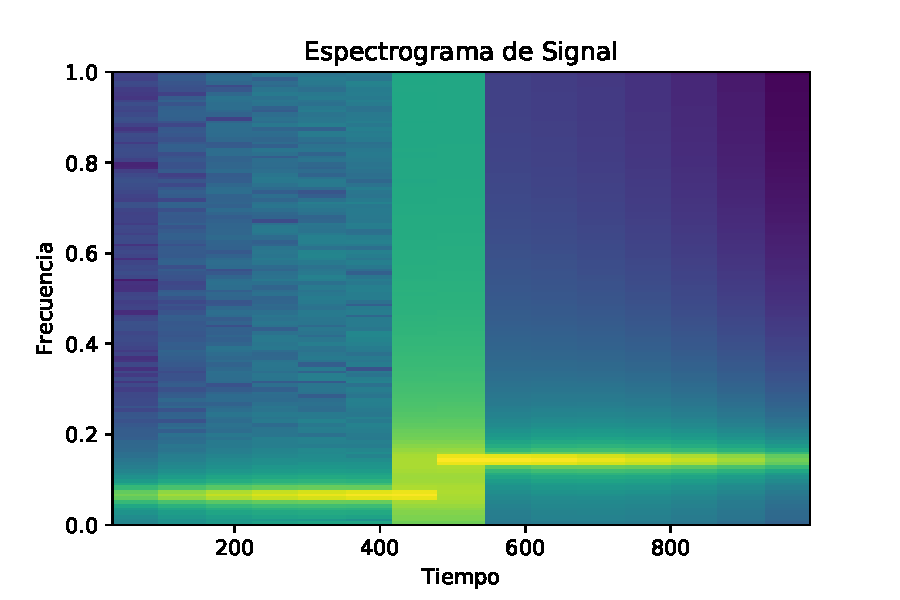
\includegraphics[width=10cm]{GarzonCamilo_espectograma_signal.pdf} 


Figura 3. Espectograma de la función signal .
\begin{flushleft}
El espectograma de la función signal muestra un cambio de la frecuencia en la mitad de la función, esto se puede explicar ya que existe una transferencia de una función a otra a la mitad de  signal.
\end{flushleft}
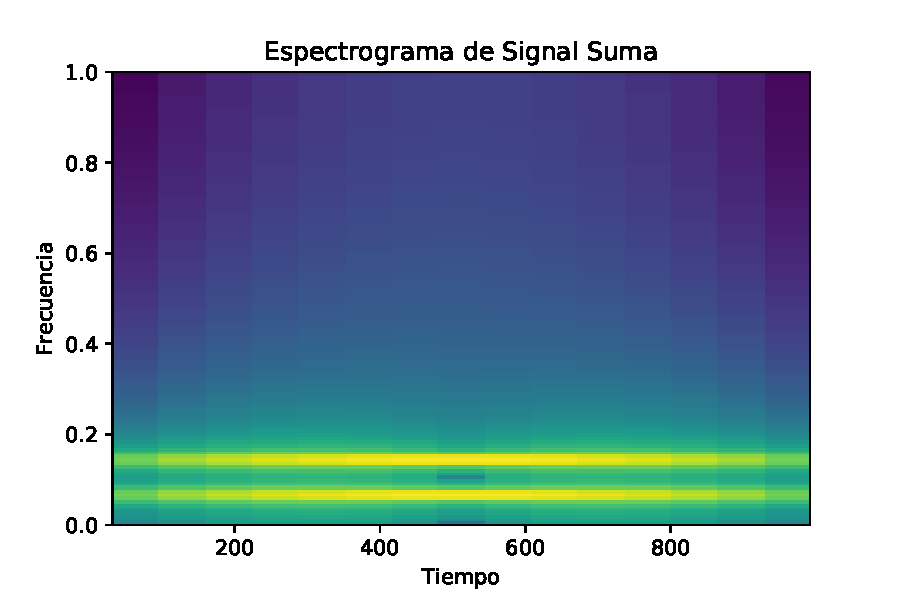
\includegraphics[width=10cm]{GarzonCamilo_espectograma_signalSuma.pdf} 


Figura 4. Espectograma de la función s signalSuma.

\begin{flushleft}
Este espectograma muestra que la funcion signal suma se mantuvo sin cambios significativos que puedan ser representados en la grafica.
\end{flushleft}
\end{center}
\vspace{5mm}
\subsection{    Gráficas usando la funcion de un temblor.} 
\vspace{5mm}
\begin{center}
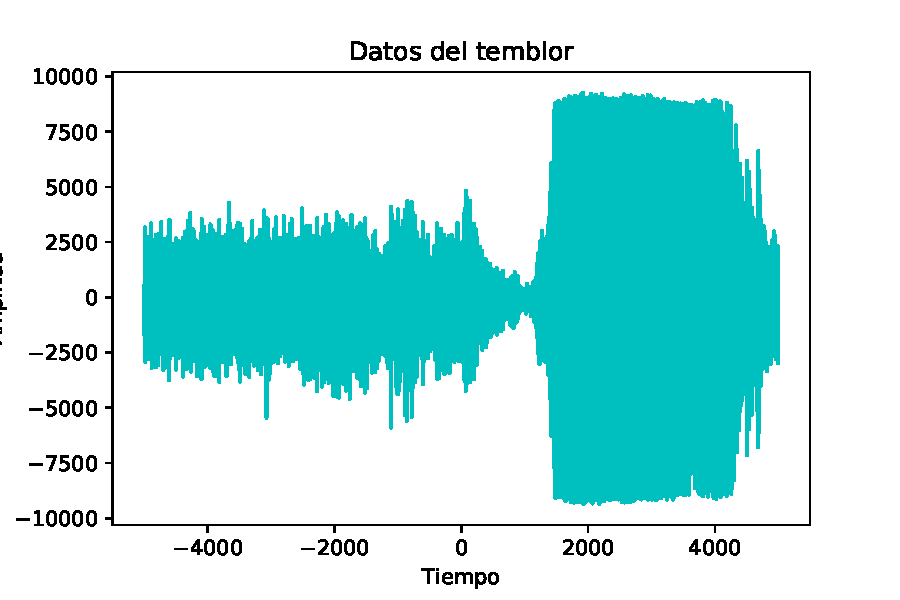
\includegraphics[width=10cm]{GarzonCamilo_temblor.pdf} 

Figura 5. Grafica temblor.

\includegraphics[width=10cm]{GarzonCamilo_TransformadasFourier_temblor.pdf} 

Figura 6. Grafica transformada discreta de fourier de la función del temblor.

\begin{flushleft}
Esta grafica muestra que la energia de la señal del temblor se almacena en los extremos con multiples picos, los cuales crecen en cuanto mas alejados esten de la frecuencia 0.
\end{flushleft}
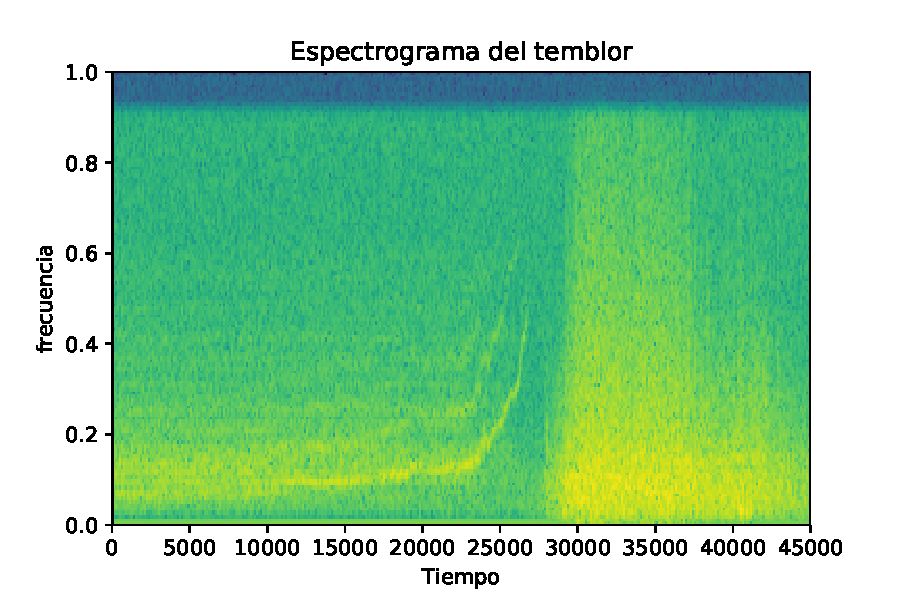
\includegraphics[width=10cm]{GarzonCamilo_espectograma_temblor.pdf} 

Figura 7. Espectograma de la función del temblor.
\begin{flushleft}
Se puede obervar que hay una franja amarilla vertical fuerte, que aparece a la mitad del espectograma. Esto en representación de los cambios de amplitud que tiene la funcion temblor, que en el caso de un temblor son provocados por movimientos de las placas tectonicas de la Tierra.
\end{flushleft}
\end{center}
\section{Ejercicio 2: Ecuaciones diferenciales sismo} 
\vspace{5mm}
\subsection{    Gráficas de las posciciones de los diferentes pisos del edifcio respecto al tiempo.} 
\vspace{5mm}
\begin{center}
\includegraphics[width=10cm]{GarzonCamilo_U1vsT.pdf} 

Figura 8. Grafica poscición de los pisos contra el tiempo w=1.9*sqrt(k/m).
\begin{flushleft}
Para este w se evidencia una resonancia poco uniforme y poco movimiento en el ultimo piso de la edificación.
\end{flushleft}
\includegraphics[width=10cm]{GarzonCamilo_U2vsT.pdf} 

Figura 9. Grafica poscición de los pisos contra el tiempo w=1.2*sqrt(k/m).
\begin{flushleft}
Para este w se evidencia una resonancia uniforme y poco movimiento en el seguno piso de la edificación.
\end{flushleft}
\includegraphics[width=10cm]{GarzonCamilo_U3vsT.pdf} 


Figura 10. Grafica poscición de los pisos contra el tiempo w=0.5*sqrt(k/m).
\begin{flushleft}
Se presenta una gran resonancia, pero no amplitudes muy altas. El ultimo piso es el que mas movimiento tiene.
\end{flushleft}
\includegraphics[width=10cm]{GarzonCamilo_U4vsT.pdf} 


Figura 11. Grafica poscición de los pisos contra el tiempo w=1.55*sqrt(k/m).
\begin{flushleft}
Con este w se presentan amplitudes muy bajas para todos los pisos y resonancias muy variantes.
\end{flushleft}
\end{center}
\vspace{5mm}
\subsection{    Gráfica de amplitud vs w.} 
\vspace{5mm}
\begin{center}
\includegraphics[width=10cm]{GarzonCamilo_UvsW.pdf} 

Figura 12. Grafica de la amplitud vs frecuencia de rozamiento.

\begin{flushleft}
Las amplitudes varian  bastante con respecto al w y hay ciertos valores donde las amplitudes llegan a un maximo, estos valores son aproximadamente w=0.6 , w=1.7 y w=2.6 esto segun las figuras de la 8 a la 12. Tambien se puede concluir que hay ciertos valores de w que hacen que la resonancia sea demasiado cambiante especificamente aquellos w que presentan amplitudes demasiadas bajas como se ve en la Figura .
\end{flushleft}
\end{center}
\end{document}

